\documentclass[11pt,a4paper]{article}
\usepackage[utf8]{inputenc}
\usepackage[T1]{fontenc}
\usepackage{amsfonts}
\usepackage[french]{babel}
\frenchbsetup{StandardLists=true} % à inclure si on utilise \usepackage[francais]{babel}
\usepackage{enumitem}
\usepackage{amssymb}
\usepackage{amsmath}
\usepackage[left=2cm,right=2cm,top=2cm,bottom=2cm]{geometry}
\usepackage{multirow}
\usepackage[dvipsnames]{xcolor}

\usepackage[T1]{fontenc}
\usepackage{fouriernc}
\usepackage{graphicx}

\usepackage{setspace}
\singlespacing

\usepackage{pstricks}
\usepackage{xkeyval}
\usepackage{pst-labo}


\usepackage{multicol}
\usepackage{caption}
\usepackage{fancyhdr}
\pagestyle{fancy}
\renewcommand\headrulewidth{1pt}
\fancyhead[L]{Lycée Denis Diderot }
\fancyhead[R]{Classe de TMICRO}
\setcounter{page}{4}\fancyfoot[C]{page \thepage}
\fancyfoot[R]{Année 2025 2026}
\fancyfoot[L]{Alexis RUIZ}
\usepackage{multirow,tabularx,booktabs}
\newcommand{\cadreblanc}[1]{%
\medskip\framebox[\linewidth][c]{%
\rule{0mm}{#1mm}}\par
\medskip}
\setlength{\columnseprule}{.25mm}

\usepackage{awesomebox}
\setlength{\aweboxvskip}{0mm}
\usepackage{pifont}
\usepackage{chemmacros}
\chemsetup{modules=all}

\renewcommand{\arraystretch}{2}
\newcommand*\acocher{\quitvmode{\fboxsep0pt \fboxrule0.8pt \fbox{\vrule height1.8ex depth.1ex width0pt \vrule height0pt depth0pt width1.9ex }}}

\newcommand{\defproblem}{\awesomebox[black]{2pt}{\rotatebox{90}{\large{\textbf{Problématique}}}}{black}}
\newcommand{\defconclusion}{\awesomebox[black]{2pt}{\rotatebox{90}{\Large{\textbf{Conclusion}}}}{black}}

\newcommand{\appel}{\awesomebox[black]{2pt}{
\includegraphics[scale=0.5]{images/appel exam.png}}{black}}

\newcolumntype{R}[1]{>{\raggedleft\arraybackslash }b{#1}}
\newcolumntype{L}[1]{>{\raggedright\arraybackslash }b{#1}}
\newcolumntype{C}[1]{>{\centering\arraybackslash }b{#1}}

\frenchbsetup{StandardLists=true}
\begin{document}



\center \LARGE{TP2 - Mesurer un niveau d'intensité acoustique}
\\[0,3cm]

\normalsize

\hrule\
\\[0,2cm]

\flushleft \textbf{NOM :\\
Prénom:\\[0,2cm]
}
\hrule\
\\[0,2cm]


\ding{202} Expérience : \\
On souhaite mesurer le niveau d'intensité acoustique en fonction de la tension d'entrée du signal. \\ [5 pt]

\ding{203} Montage : Ajout d'un voltmètre.\\
Sur le montage ci-dessous, schématiser un voltmètre permettant de mesurer la tension d'entrée du signal émise par le haut parleur. \\
\begin{center}
\hspace{2cm}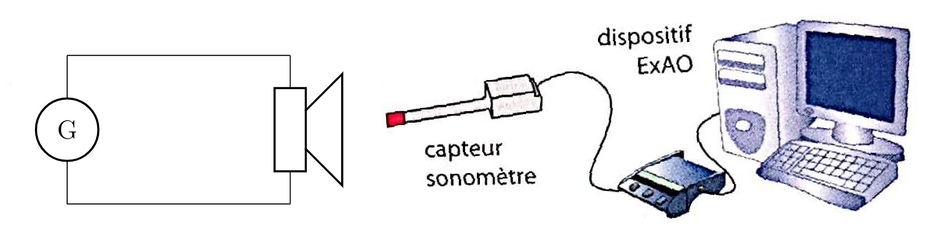
\includegraphics[scale=1.3]{images/TP2 - montage.jpg} 
\end{center}

\appel{\fbox{
\begin{minipage}{14cm}{
\begin{center}
 Appeler le professeur pour pour qu'il vérifie votre schéma.
 \end{center} }

\end{minipage}
}}
\vspace{5mm}

\ding{204} Expérience:\\
\begin{itemize}
	\item Réaliser le montage ci-dessus
	\item Régler le GBF sur le signal sinusoïdal avec une fréquence de 1000 Hz et une tension de 0,1 V.\\[5pt]
	
	\appel{\fbox{
\begin{minipage}{12cm}{
\begin{center}
 Appeler le professeur pour pour qu'il vérifie les réglages et règle la console d'acquisition.
 \end{center} }

\end{minipage}
}}

	\item Compléter le tableau suivant en modifiant la valeur de la tension. 
	
\begin{center}
	\begin{tabular}{|C{1.5cm}|C{1.5cm}|C{1.5cm}|C{1.5cm}|C{1.5cm}|C{1.5cm}|C{1.5cm}|}
	\hline 
	U(V) & 0,1& 0,3~~ & ~~0,5~~ & 0,7 & 1 & $U_{max}$\\ 
	\hline 
	L(dB) &   &   &   &   & & \\ 
	\hline 
	\end{tabular} 
\end{center}

    \item Imprimer votre graphique (à rendre avec la copie)
	
\end{itemize}
\ding{205} Conclusion :\\
Qu'observez vous lorsque la tension du GBF augmente ? \\[5 pt]
\cadreblanc{25}
\end{document}